Al colocar a un resorte distintos pesos su longitud aumenta; así es como funciona
un dinamómetro. Llamemos alargamiento a la distancia que aumenta la longitud del resorte al colocarle un peso;
este comportamiento del resorte se conoce como la \emph{ley de Hooke}.

\begin{multicols}{2}
    \begin{parts}
        \part Ubica en el plano cartesiano de la Figura \ref{fig:} los
        puntos $\left(0, 6\right)$, $\left(\frac{1}{2},7\right)$, $\left(1, 8\right)$ y $\left(2, 10\right)$ que indican el peso
        que se colocó al resorte y su longitud total.


        % \begin{minipage}[t][5cm][b]{0.3\textwidth}
        \begin{figure}[H]
            \centering
            \ifprintanswers
                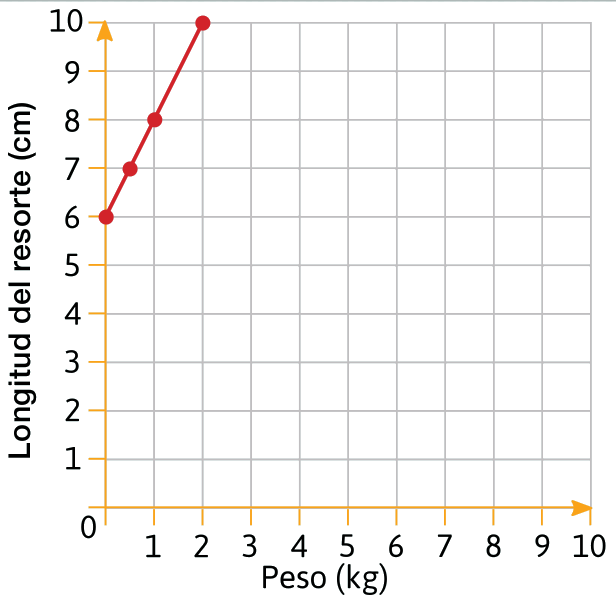
\includegraphics[width=.65\linewidth]{../images/20230320215617}
            \else
                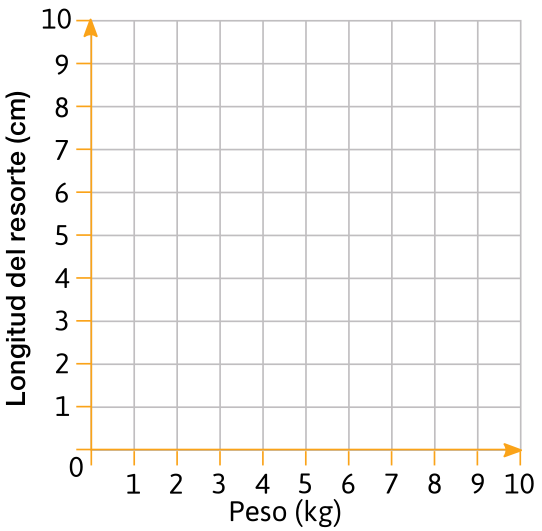
\includegraphics[width=.65\linewidth]{../images/20230320205645}
            \fi
            \caption{Plano cartesiano}
            \label{fig:20230320205645}
        \end{figure}

        \part ¿En qué punto interseca esa línea el eje vertical?

        \begin{solutionbox}{1.2cm}
            En el punto (0, 6).
        \end{solutionbox}

        \columnbreak

        \part Une los puntos en la gráfica. ¿Qué tipo de línea trazaron?

        \begin{solutionbox}{1.2cm}
            Es una línea recta.
        \end{solutionbox}



        \part ¿Cómo aumenta la longitud del resorte al aumentar el peso?

        \begin{solutionbox}{1.6cm}
            Aumenta 2 cm por cada kilogramo de peso que se agrega.
        \end{solutionbox}

        \part ¿La longitud del resorte es proporcional al peso que se le aplica? \emph{Explica tu respuesta}

        \begin{solutionbox}{1.6cm}
            Si, la razón de la longitud del resorte entre el peso que se le coloca es constante.
        \end{solutionbox}
    \end{parts}
\end{multicols}
% \begin{minipage}[t]{0.25\textwidth}

% \end{minipage}\hfill
% \begin{minipage}[t]{0.5\textwidth}

% \end{minipage}
